%%%%%%%%%% Prefix a "S" to all equations, figures, tables and reset the counter %%%%%%%%%%
\setcounter{equation}{0}
\setcounter{figure}{0}
\setcounter{table}{0}
\setcounter{page}{1}
\makeatletter
\renewcommand{\thefigure}{S\arabic{figure}}
%%%%%%%%%%%%%%%%%%%%

\section{Mathematical derivations}


\section{Supplementary Figures}

\begin{figure}[tbph]
    \subfloat[]{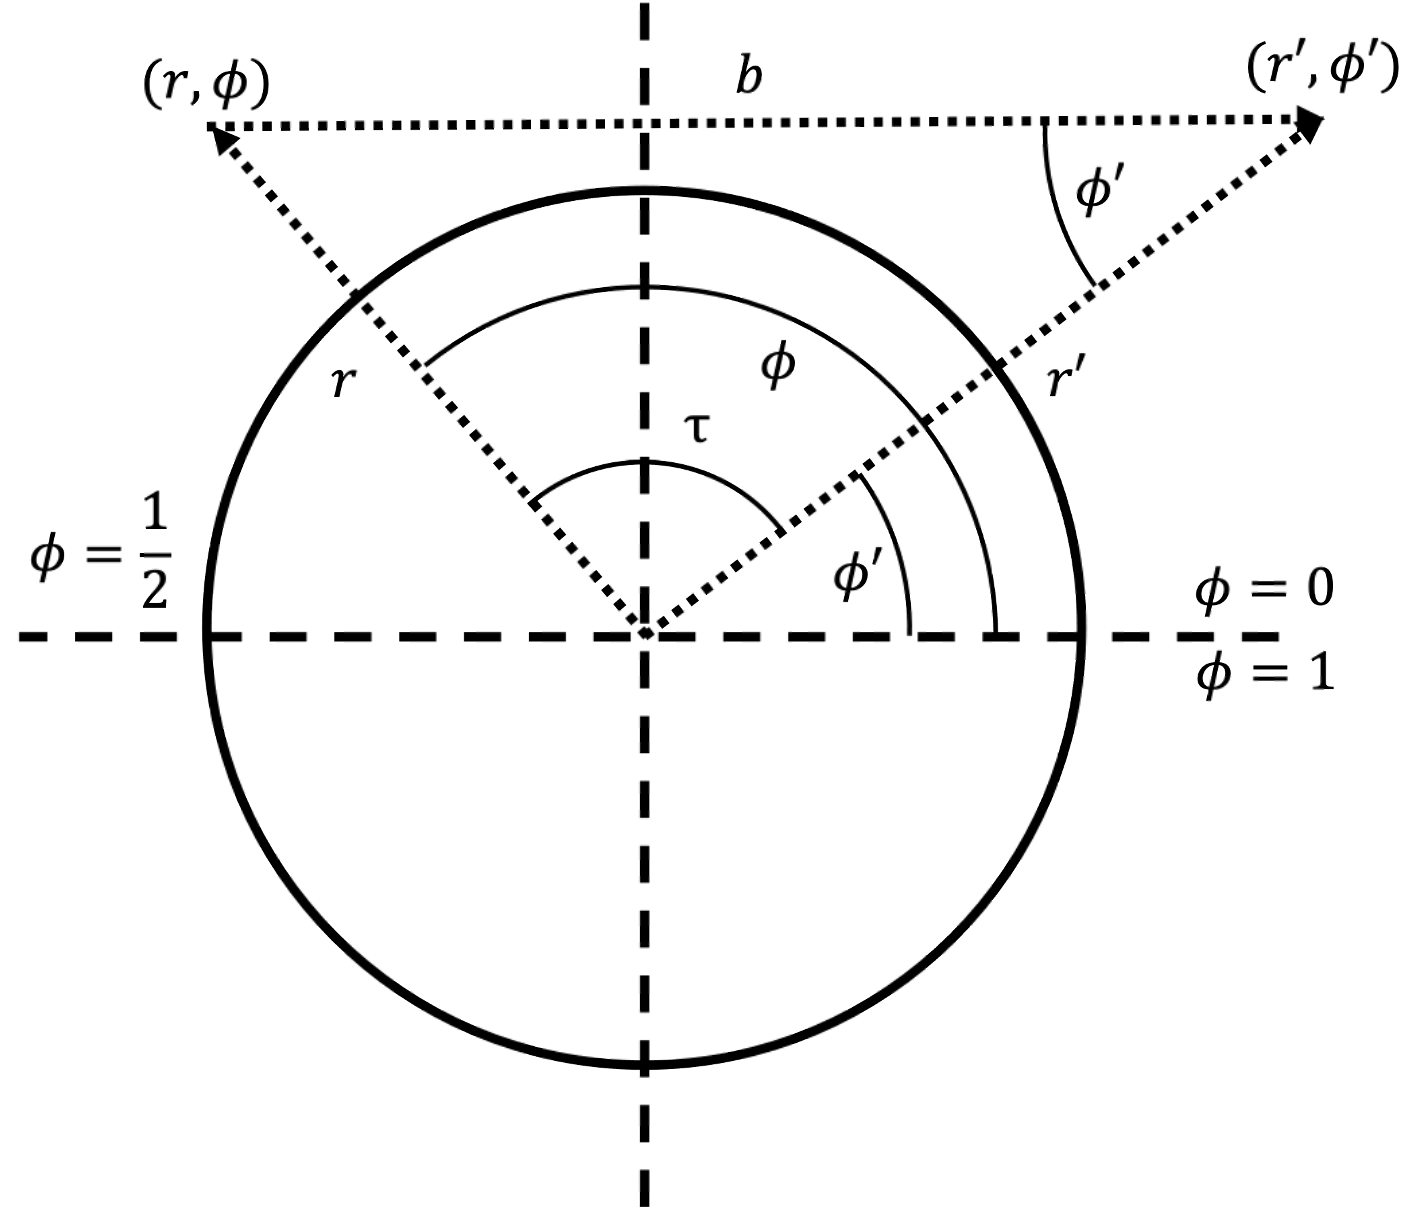
\includegraphics[width=0.45\textwidth]{figures/Fig4.png}\label{fig:a}}
    \medskip
    \subfloat[]{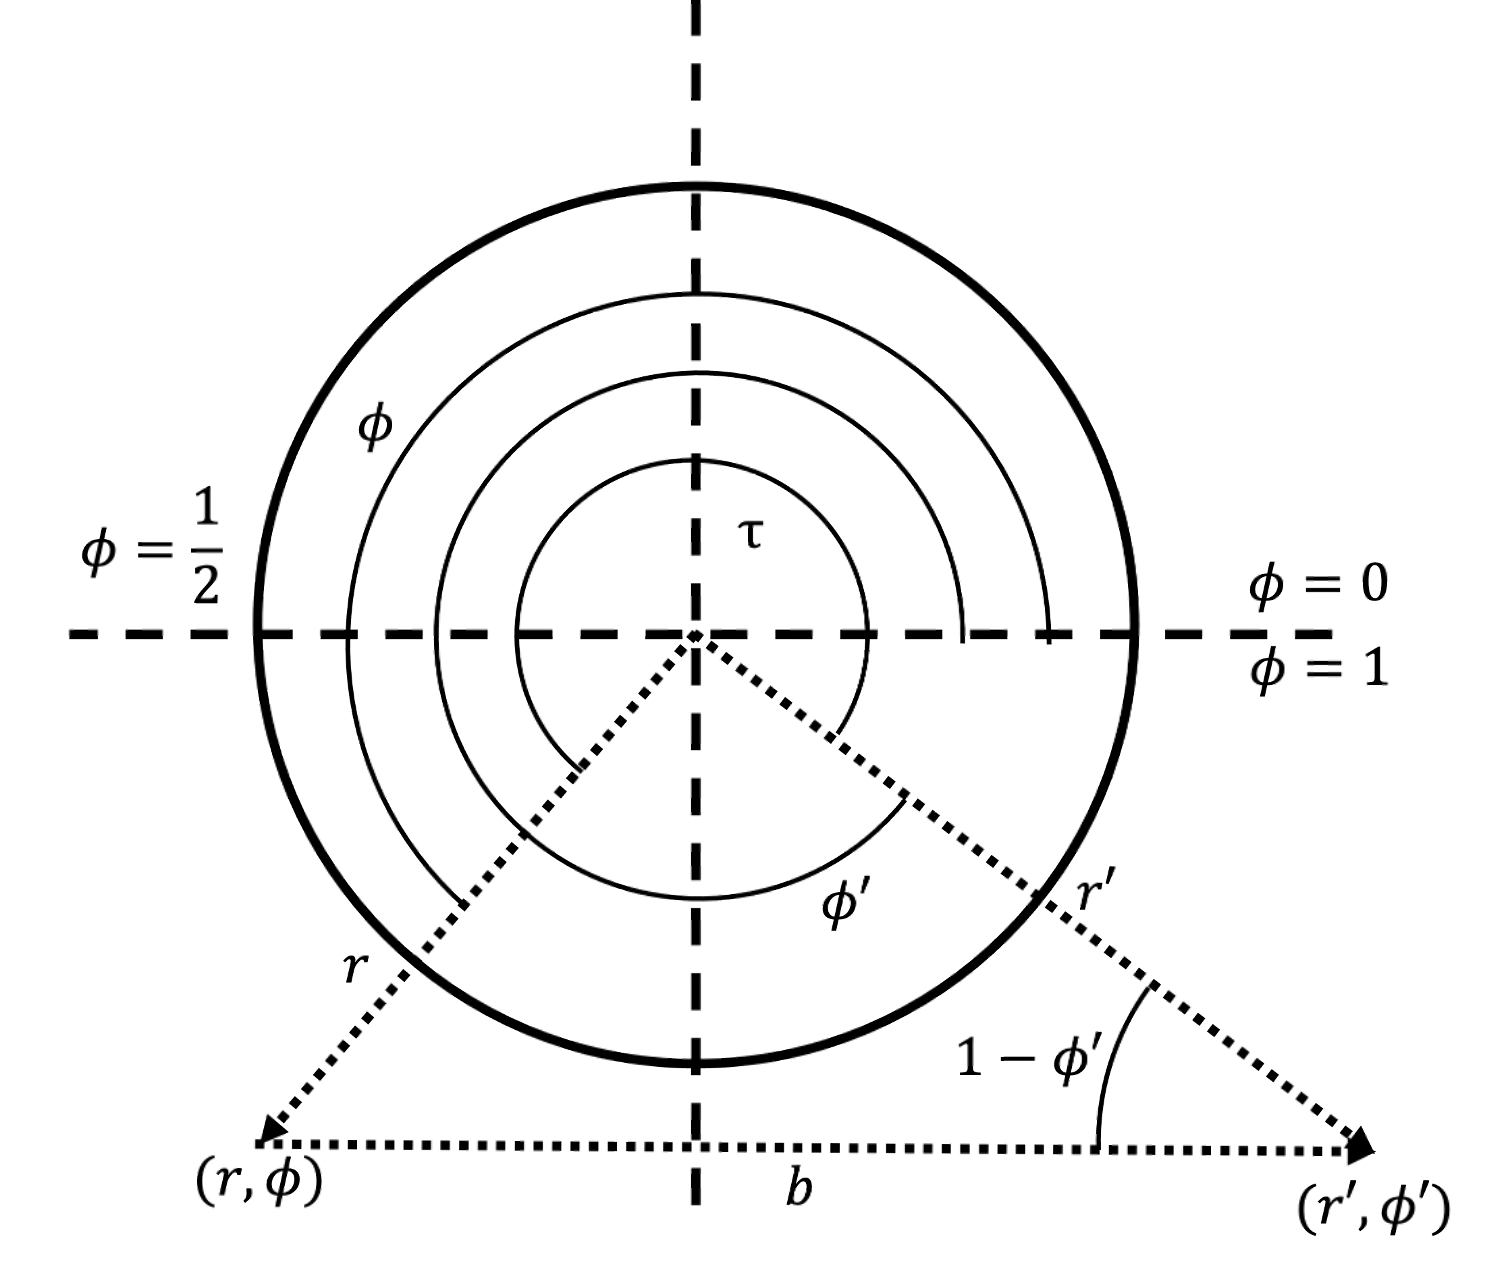
\includegraphics[width=0.45\textwidth]{figures/Fig4-2.png}\label{fig:b}}
    \caption{\textbf{For the period-1 cycle, we can write $\tau = \phi_i - \phi'_i$ for $0\leq \phi \leq1/2$ and $\tau = 1-(\phi'_i - \phi_i)$ for $1/2\leq \phi \leq1$. Fig a) Fig b)}}
    \label{sines}
\end{figure}


\begin{figure}[H]
    \begin{center}
    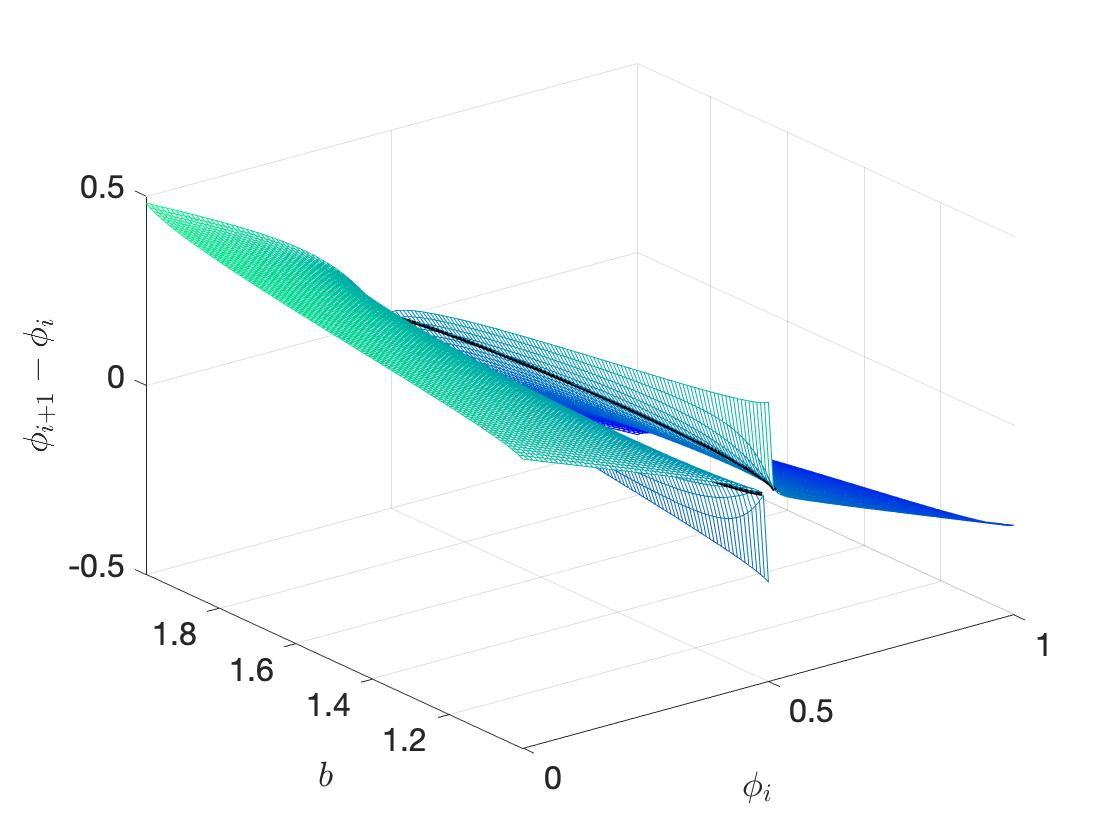
\includegraphics[width=.8\textwidth]{figures/3dplot1.jpg}
    \end{center}
\caption{The blue surface is Eq.(\ref{eq:right}). The black line is Eq.(\ref{eq:square}) where $\phi_{i+1}=\phi_i$. Eq.(\ref{eq:right}) intersects fully Eq.(\ref{eq:square}) where the period-1 condition ($\phi_{i+1}=\phi_i$) is satisfied.}
\label{instabbound}
\end{figure}


\begin{figure}
    \begin{center}
    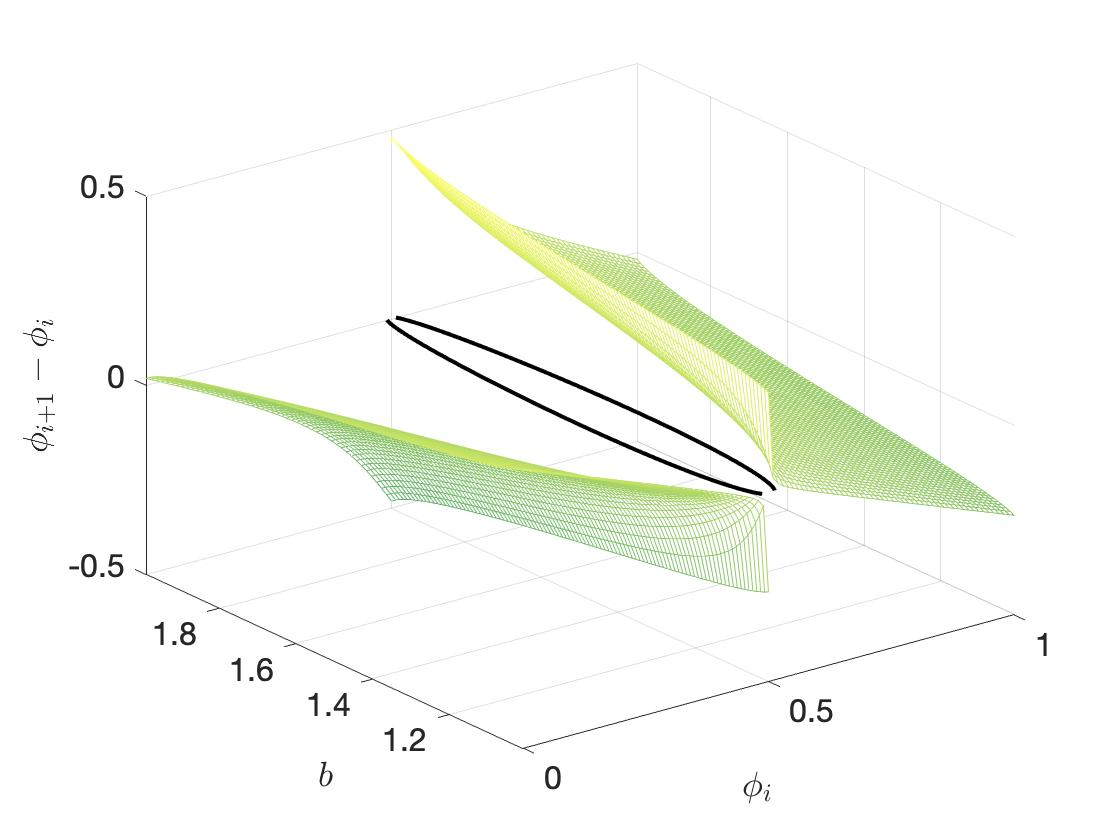
\includegraphics[width=.8\textwidth]{figures/3dplot2.jpg}
    \end{center}
    \caption{The green surface is Eq.(\ref{eq:wrong}). The black line is Eq.(\ref{eq:square}) where $\phi_{i+1}=\phi_i$. Eq.(\ref{eq:wrong}) does not intersect Eq.(\ref{eq:square}) anywhere the period-1 condition ($\phi_{i+1}=\phi_i$) is satisfied.}
    \label{instabbound_restric}
\end{figure}